%  
%                 TROPOSFERA
%  

\chapter{Qu\'{\i}mica de la troposfera}
\index{troposfera!quimica@química}

\section{Especies oxidantes en la troposfera}
Varios de los gases de importancia en la atmósfera se remueven principalmente mediante la oxidación: Los gases de efecto invernadero como el metano, los gases producto de la combustión como el CO, los compuestos que destruyen el ozono estratosférico como los HFC y otros. La oxidación en la troposfera es de importancia clave por que la troposfera contiene la masa principal de la atmósfera (85\%) y los compuestos traza se emiten principalmente en la superficie.

Los oxidantes mas abundantes en la atmósfera terrestre son el oxígeno y el ozono. Esos oxidantes poseen energías de enlace grandes y que relativamente no reactivos excepto con los radicales. Con pocas excepciones, la oxidación de especies no radicales con el \ce{O2} y \ce{O3} son muy lentas. Se ha identificado que el radical OH reacciona rápidamente con la mayoría de de las especies no radicales y particularmente reacciona con moléculas conteniendo H debido a la reacción de abstracción de H convirtiendo el OH en \ce{H2O}. 

\subsection{Radical Hidroxilo}
\index{radical!hidroxilo}

La producción de OH es mediante la reacción de vapor de agua con \ce{O(^1D)}

\reaction{O3 + h$\nu$ ->[k_1] O2 + O(^1D) \label{OHR1} }
\reaction{O(^1D) + M ->[k_2] O2 + M \label{OHR2} }
\reaction{O(^1D) + HO2 ->[k_3]  2OH  \label{OHR3} }

Una expresión simple entre las reacciones \ref{OHR1} y \ref{OHR3}  para la generación del OH  ($P_\mathrm{OH}$) 
\begin{equation}
P_\mathrm{OH}= 2k_3 [\ce{O(^1D)}] [\ce{H2O}] = \frac{2k_1k_3}{k_2[\mathrm{M]}+k_3[\ce{H2O}]} [\ce{O3}][\ce{H2O}] 
\end{equation}
En experimentos se ha encontrado que la reacción \ref{OHR2} es mucho mas rápida que la \ref{OHR3} simplificando:

\begin{equation}
P_\mathrm{OH} \approx  \frac{2k_1k_3}{ k_2[M] } [\ce{O3}]  [\ce{H2O}] 
\end{equation}

Una parte crítica en la generación del OH es la producción de átomos de  \ce{O(^1D)}  mediante \ref{OHR1}. 

\subsubsection{Producci\'on en la troposfera de OH}
La producción troposférica de \ce{O(^1D)} toma lugar en una  banda angosta de longitudes de onda entre 300 y 320 nm; la radiación de ondas más cortas no penetra en la troposfera, mientras que longitudes de onda mayores no se absorbe por el \ce{O3}. Aunque la producción de \ce{O(^1D)} es mucho menor en la troposfera que la estratosfera, esto se ve compensado en términos de la producción de OH por cantidades mayores de \ce{H2O} en la troposfera. Cálculos con modelos considerando la penetración de radiación UV entre 300-320 \nano\metre\,  encontró que las concentraciones de OH en el orden de $10^6$ moléculas/\cubic\metre, resultando en que el CO tiene un tiempo de vida en la troposfera de algunos meses.
\subsubsection{La concentraci\'on global media del OH}
El tiempo de vida del OH en una parcela de aire esta dado por:
\begin{equation*}
\tau=\frac{1}{\sum k_in_i}
\end{equation*}
donde $n_i$ es la densidad numérica de las especies $i$ que reacciona con el OH, $k_i$, es la constante de rapidez  correspondiente. Se ha identificado que el CO es el sumidero dominante del OH en la mayoría de la troposfera, y el \ce{CH4} es el segundo en importancia. El resultado del tiempo de vida del OH es del orden de un segundo. Debido a este tiempo de vida corto, las concentraciones del OH son muy variables.

La estimación del  $\overline{[\mathrm{OH}]}$ se realizó mediante el uso del solvente metilcloroformo (\ce{CH3CCl3}) con base en su emisión y pérdidas se estima que la concentración media del  $\overline{[\mathrm{OH}]}$ es de $1.2\times10^6$ moléculas/\centi\cubic\metre.

Esta estimación empírica del   $\overline{[\mathrm{OH}]}$ es útil por que puede emplearse para estimar la vida  $\tau=1/(k_i/(\overline{[\mathrm{OH}]})$ de cualquier gas $i$ con la oxidación por el OH en la troposfera. Así el \ce{CH4} posee una vida de 9 años y el \ce{CH3Br} de dos años.

En la Ciudad de México durante la campaña MCMA-2003 se midieron concentraciones de OH en promedio de  $3.78\times10^6$ con picos de $180\times10^6$ moléculas/\centi\cubic\metre.

\subsection{Ciclado de HO$_x$ y producci\'on de ozono}
\subsubsection{Mecanismo de oxidaci\'on del CO}\label{ciclado}

La oxidación del CO por OH produce un átomo de H, el cual reacciona rápidamente con el \ce{O2}:
\begin{eqnarray}
\ce{CO + OH & -> &CO2 + H} \label{OHR4}  \\
\ce{H + O2  & ->[M]  & HOO^.}  \label{OHR6} 
\end{eqnarray}

El radical resultante \ce{HO2} puede reaccionar consigo mismo para producir peróxido de hidrógeno (\ce{H2O2}):

\reaction{ HOO^. + HOO^. -> H2O2 + O2 \label{OHR7}}

El peróxido de hidrógeno es muy soluble en agua y se remueve de la atmósfera por depositación en una escala de tiempo de una semana. También  se  fotoliza o puede  reaccionar con el OH:
\reaction{ H2O2 + h$\nu$ -> 2OH \label{OHR8}}
\reaction{ H2O2 + OH -> HO2 + H2O \label{OHR9}}
La reacción \ref{OHR8} regenera OH mientras que la \ref{OHR9} consume un OH adicional.

En presencia de NO, una reacción alternativa del \ce{HO2} es
\reaction{ HOO^. + NO  -> OH + NO2 \label{OHR10}}
la cual regenera el OH y también produce \ce{NO2} el cual continúa fotolizando:
\reaction{ NO2 + O2  + h$\nu$ -> NO + O3 \label{OHR11} } 
La reacción\,\ref{OHR11} regenera el NO y produce una molécula de \ce{O3}, la cual se puede fotolizar en las reacciones \ref{OHR1}--\ref{OHR3} para producir dos moléculas adicionales de OH. Por lo tanto, la reacción \ref{OHR10} produce tres moléculas de OH, incrementado el poder oxidativo de la atmósfera. La secuencia de reacciones \ref{OHR4} + \ref{OHR6} + \ref{OHR10} + \ref{OHR11} es un mecanismo de reacción para la producción de \ce{O3} en el que se cataliza la oxidación de CO con \ce{O2} por la familia del  \ce{HO_$x$} (\ce{HO_$x$= H + OH + HO2})  y por \ce{NO_$x$}.

El resultado neto de la reacción es:
\reaction*{CO + 2O2 -> CO2 + O3}
\begin{figure}[htbp]
\begin{center}
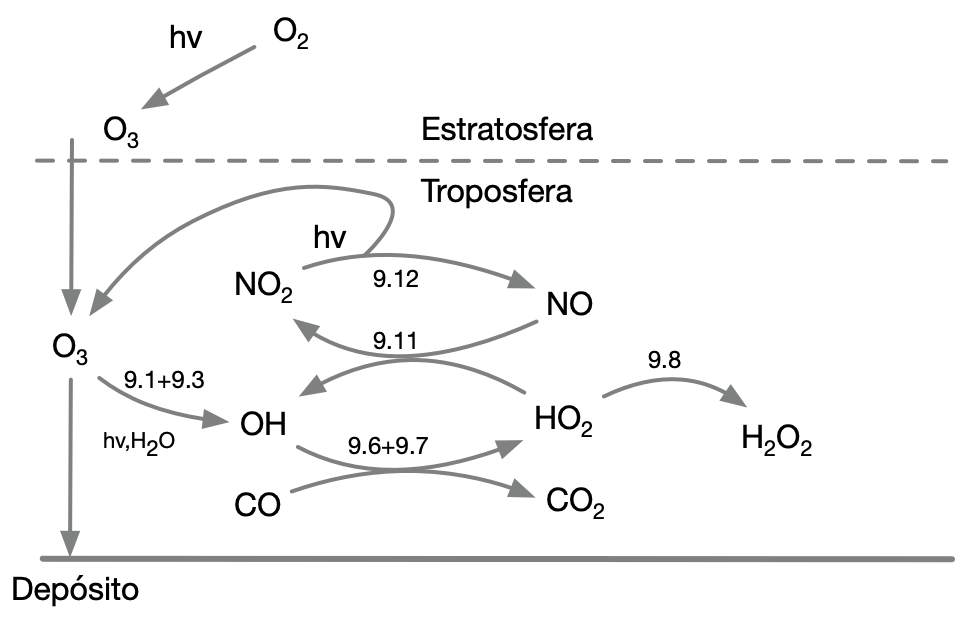
\includegraphics[width=0.95\textwidth]{CO_oxidacion.png}
\caption{Ciclo de oxidación del CO}
\label{CO_ox}
\end{center}
\end{figure}

En la \textbf{Figura~\ref{CO_ox}} se puede observar que la cadena se inicia por la fuente de \ce{HO_$x$} de la reacción~\ref{OHR3}, y se termina por la pérdida de radicales \ce{HO_$x$} mediante \ref{OHR7}. La eficiencia de propagación del mecanismo (longitud del mecanismo) se determina por la abundancia del \ce{NO_$x$}.

Es notable observar que el \ce{HO_$x$} y el \ce{NO_$x$} catalizan la producción de \ce{O3} en la troposfera y la destrucción de \ce{O3} en la estratosfera. La principal diferencia entre la troposfera y la estratosfera es que concentraciones de \ce{O3} y O son mucho menores en la troposfera.

\subsubsection{Mecanismo de oxidaci\'on del metano (\ce{CH4})}

El mecanismo de oxidación del metano involucra mas pasos que la oxidación del CO pero sigue el mismo esquema. El radical metilo (\ce{CH3}) se producido por la oxidación inicial rápidamente adiciona \ce{O2}:
\reaction{ CH4 + OH -> CH3 + H2O \label{OHR5} }
\reaction{  CH3 + O2 ->[M] CH3O2 \label{OHR16}} 
El radical metilperoxi (\ce{CH3O2})\index{radical!metilperoxi} es análogo al \ce{HO2} y se considera parte de la familia \ce{HO_$x$}. Su principal sumidero son las reacciones de  \ce{HO2}  y NO:
\reaction{CH3O2 + HO2 -> CH3OOH + O2 \label{OHR17}}
\reaction{ CH3O2 + NO -> CH3O + NO2\label{OHR18}}

El metilhidroperoxido (\ce{CH3OOH})\index{metilhidroperoxido} puede reaccionar con el OH o fotolizarse. La reacción con el OH posee dos ramas debido a la abstracción del H que puede tener lugar tante en el lugar del metilo o en el grupo hidroperoxi. El radical  \ce{CH2OOH} producido por la primera rama se descompone rápidamente a formaldehído (HCHO) y OH:

\reaction{ CH3OOH + OH -> HCHO + OH + H2O \label{OHR19}}
\reaction{ CH3OOH + OH -> CH3O2 + H2O          \label{OHR20}}
\reaction{ CH3OOH + h$\nu$ -> CH3O + OH        \label{OHR21}}

El radical metoxi (\ce{CH3O}) producido por las reacciones \ref{OHR18} y \ref{OHR21} va a reaccionar rápidamente con \ce{O2}:
\reaction{ CH3O + O2 -> CH2O + HOO        \label{OHR22}}
y el \ce{HO2} reacciona  como se describió en la sección anterior (\ref{ciclado}).

El formaldehído producido en \ref{OHR22} puede tanto reaccionar con el OH o fotolizarse (dos ramas de fotólisis):
\reaction{ HCHO + OH -> CHO + H2O          \label{OHR23}}
\reaction{ HCHO + h$\nu$ +O2 -> CHO + HO2          \label{OHR24}}
\reaction{ HCHO + h$\nu$ -> CO + H2          \label{OHR25}}

Las reacciones~\ref{OHR23} y~\ref{OHR25} producen el radical CHO, el cual reacciona con el \ce{O2} y conduce al CO y \ce{HO2}:
\reaction*{CHO + O2 -> CO + HO2}
El CO se oxida a \ce{CO2} mediante el mecanismo descrito anteriormente (Reacción~\ref{OHR4}).

En esta secuencia general de reacciones el átomo de \ce{C^{-IV}} en el \ce{CH4} (el menor estado de oxidación del carbono) se oxida sucesivamente de \ce{C^{-II}} en \ce{CH3OOH}, \ce{C^{0}} en \ce{CH2O}, \ce{C^{+II}} en CO y \ce{C^{+IV}} en \ce{CO2}  (el mayor estado de oxidación del carbono). La producción de ozono se da por la fotólisis del \ce{NO2} seguido de las reacciones peroxi + NO: \ref{OHR10} y \ref{OHR18}, donde los radicales peroxi se generan por reacciones \ref{OHR5} + \ref{OHR16} , \ref{OHR20}, \ref{OHR22}, \ref{OHR24}, \ref{OHR25} y \ref{OHR4} + \ref{OHR6}.
\begin{description}
\item[Atmósfera con alta concentración de \ce{NO_$x$}]
En un régimen de alto NOx se llega a la reacción neta de conversión del \ce{CH4} a \ce{CO2}:
\reaction*{CH4 + 10O2 -> CO2 + H2O + 5O3 + 2OH }
dando una producción total de cinco moléculas de \ce{O3} y dos moléculas de OH por cada molécula de \ce{CH4} oxidada.
\item[Atmósfera con baja concentración de \ce{NO_$x$}]
En una atmósfera desprovista de \ce{NO_$x$} el mecanismo nos lleva a la reacción neta:
\reaction*{CH4 + 3OH + 2O2 -> CO2 + 3H2O + HO2 }
así el \ce{O3} no se produce y dos moléculas de OH se consumen. Este resultado enfatiza de nuevo el papel crítico del \ce{NO_$x$} para mantener las concentraciones de \ce{O3}  y OH en la troposfera.

La oxidación de hidrocarburos mayores sigue el mismo tipo de mecanismo como el \ce{CH4}. Esos hidrocarburos posee fuentes similares a las del metano y son por lo tanto menos importantes que el \ce{CH4} en la química troposférica global. Sin  embargo estos son críticos en la producción rápida de \ce{O3}  en regiones contaminadas y tiene un rol importante en el transporte a larga distancia del \ce{NO_$x$}.
\end{description}

\subsection{Estimaci\'on global de los óxidos de nitrógeno }
\index{nitrogeno@nitrógeno!oxidos@óxidos}

De las fuentes de \ce{NO_$x$} en las condiciones actuales la combustión de combustibles fósiles representa la mitad las fuentes globales. La quema de biomasa, de la agricultura y deforestación tropical, representa un 25\%. Parte de la fuente de combustión es debido a la oxidación de nitrógeno presente en el combustible. Una fuente adicional en la combustion de motores es la descomposición térmica del aire alimentado a la cámara de combustion. En altas temperaturas de combustion ($\sim 2000\kelvin$), el oxígeno se termoliza y reacciona subsecuentemente la reacción del O con \ce{N2} para producir NO:
\reaction{ O2  <=>[][\triangle] O^. + O^. \label{OHR27}}
\reaction{ N2 + O^. <=> NO + N^. \label{OHR28}}
\reaction{ N^.  + O2 <=>  NO + O^. \label{OHR29}}
El equilibrio de \ref{OHR27} a \ref{OHR29} se desplaza a la derecha a altas temperaturas, promoviendo la formación de NO. El mismo mecanismo térmico también conduce a la emisión de NO por rayos, ya que el aire dentro del canal del rayo se calienta a temperaturas extremadamente altas. Otras fuentes menores de \ce{NO_$x$}, \textbf{Cuadro~\ref{noxt}} , incluyen la nitrificación y desnitrificación bacteriana del suelo, la oxidación del  \ce{NH3} emitido por la biosfera, del transporte de la estratosfera del \ce{NO_$y$}  producido por la oxidación del \ce{N2O}  por el \ce{O(^1D)}. La oxidación del \ce{N2O}  no toma lugar en la troposfera debido a que la concentración del \ce{O(^1D)} es muy baja.
\begin{table}[htp]
\caption{Emisiones estimadas de \ce{NO_$x$} troposférico}
\begin{center}
\begin{tabular}{|l|c|}\hline
Fuente & \tera\gram/año \\\hline
Combustión de combustibles fósiles&	21 \\
Quema de biomasa	&12  \\
Suelos&	6 \\
Relámpagos&	3 \\
Oxidación de \ce{NH3} &	3 \\
Aviación&	0.5 \\
Transporte de la estratosfera&	0.1 \\\hline
\end{tabular}
\end{center}
\label{noxt}
\end{table}%
A pesar de que el \ce{NO_$x$} se emite principalmente como NO, el ciclado entre NO y \ce{NO2} toma lugar en la troposfera en escala de tiempo de un minuto durante el día por \ref{R10} y \ref{R11} y mediante el ciclo nulo\index{ciclo nulo}:
\reaction{ NO + O3 -> NO2 + O2 \label{NOR14}}
\reaction{ NO2 + h$\nu$ ->[O2] NO + O3 \label{NOR11}}

Debido a este ciclado rápido, es mas apropiado considerar la cantidad de la familia \ce{NO_$x$}  en su conjunto, como en la estratosfera. Por la noche, el \ce{NO_$x$}  se presenta exclusivamente como \ce{NO2} como resultado de \ref{NOR14}.

La actividad humana claramente es la mayor fuente de \ce{NO_$x$} en la troposfera. pero  pero cuantificar el alcance global de la influencia humana sobre las concentraciones de \ce{NO_$x$} es difícil porque la vida útil de los \ce{NO_$x$} es muy corta. El sumidero principal del \ce{NO_$x$} es la oxidación a \ce{HNO3}\index{no3@\ce{NO3}}, como en la estratosfera; en el día 
\reaction{ NO2 + OH ->[M] HNO3 + O2 \label{NOR30}}
y durante la noche,
\reaction{ NO2 + O3 -> NO3 + O2    \label{NOR31}}
\reaction{ NO3 + NO2  ->[M] N2O5  \label{NOR32}}
\reaction{ N2O5 + H2O  -> 2HNO3  \label{NOR33}}

El tiempo de vida resultante del \ce{NO_$x$} es aproximadamente un día. En la estratosfera, observamos que el \ce{HNO3} se recicla hacia el \ce{NO_$x$} por la fotólisis y reacción con el OH en una escala de tiempo de unas semanas. En la troposfera, sin embargo, el \ce{HNO3} es removido por la precipitación{on debido a su alta solubilidad en agua. El tiempo de vida de especies solubles en agua contra la deposición es típicamente de pocos días en la troposfera baja y de pocas semanas en la troposfera superior. Se concluye que el \ce{HNO3} en la troposfera se remueve principalmente por la deposición y no es un reservorio para el \ce{NO_$x$}.

Se ha observado que un mecanismos más eficiente para el transporte a largas distancia de \ce{NO_$x$} antropogénico en la troposfera global es mediante la formación de otras especies repertorio, el peroxiacetilnitrato (\ce{CH3C(O)OONO2})\index{PAN}. El prexiacetilnitrato (llamado PAN) es producido en la troposfera por la oxidación fotoquímica de compuestos carbonilos en presencia de \ce{NO_$x$}. Esos carbonilos son producidos por la oxidación fotoquímica de hidrocarburos emitíos por una variedad de fuentes biogénicas y antropogénicas. En el caso simple de acetaldehido (\ce{CH3CHO}), en la formación de PAN se da de la siguiente forma:

\reaction{ CH3CHO + OH  -> CH3CO  + H2O \label{NOR34}}
\reaction{ CH3CO + O2  ->[M] CH3C(O)OO^.   \label{NOR35}}
\reaction{ CH3C(O)OO^.  + NO2  ->[M] PAN   \label{NOR36}}

La formación de PAN es generalmente menos importante como sumidero para \ce{NO_$x$}  que la formación de \ce{HNO3}. Sin embargo, en contraste con el \ce{HNO3}, PAN es poco soluble en agua y no se remueve por depositación. Su principal pérdida es por la descomposición térmica, regenerando \ce{NO_$x$} :
\reaction{ PAN ->[][\triangle]  CH3C(O)OO^.  + NO2 \label{NOR37}}
El tiempo de vida del PAN (reacción~\ref{NOR37}) es de sólo una hora a $295\kelvin$ pero de varios meses a $250\kelvin$; notar la fuerte dependencia a la temperatura. En la baja troposfera, \ce{NO_$x$}  y PAN se encuentran típicamente cerca del equilibrio químico. En la troposfera media y superior, sin embargo, el PAN puede transportarse sobre largas distancias y descomponerse liberando \ce{NO_$x$}  lejos de su fuente.
\begin{figure}[htbp]
\begin{center}
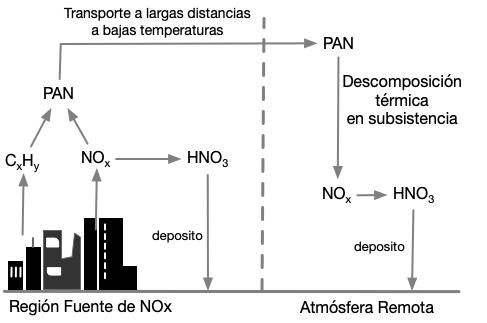
\includegraphics[width=0.85\textwidth]{PAN.png}
\caption{Transporte de NO$_x$ por PAN}
\label{noxpan}
\end{center}
\end{figure}

\subsection{Reacciones del radical NO$_3$}
\index{radical!nitrato@\ce{NO3}!reacciones}
El radical nitrato (\ce{NO3}) se forma por la reacción~\ref{NOR31} entre el \ce{O3} y \ce{NO2},  y tiene un papel importante en la química atmosférica nocturna del aire contaminado. El \ce{NO3} posee un espectro de absorción en la región visible por lo que su concentración durante el día es muy baja debido a que es fácilmente fotolizado por la luz solar. Simultáneamente, debido a que la contante de reacción del \ce{NO3} con el NO es grande, se regenera fácilmente a \ce{NO2} por el NO así su concentración cerca de las fuentes de NO es muy baja. El \ce{NO3} reacciona con alquenos y aldehídos para formar dinitratos y radicales OH/\ce{HO2} durante la noche. 
\begin{description}
\item[\ce{NO3 + NO} ] 
La reacción del \ce{NO3}  y NO es una transferencia simple de un átomo de oxígeno,
\reaction{ NO3 + NO  -> 2NO2  \label{NOR38}}
Esta reacción es rápida.
\item[\ce{NO3 + NO2 + M} ] 
La reacción  (\ref{NOR32}) de los radicales \ce{NO3}  y \ce{NO2}  en la atmósfera contaminada durante la noche elimina el \ce{NO3}  para formar \ce{N2O5}, que se transforma en ácido nítrico, \ce{HONO2}, al reaccionar con \ce{H2O}. Por lo tanto, esta reacción es importante como un proceso que elimina \ce{NO_$x$}  del sistema de reacción en cadena y forma un reservorio \ce{HONO2} junto con la reacción diurna de \ce{OH + NO2 + M}

La vida atmosférica del \ce{N2O5}  a temperatura ambiente y presión atmosférica es de aproximadamente 10\second, y durante esta vida, el \ce{N2O5} se convierte en \ce{HONO2} mediante una reacción homogénea con la molécula de  \ce{H2O}, o heterogénea con aerosoles (como en reacción~\ref{NOR33}).
\item[\ce{NO3   +  C2H4} ] 
Se sabe que los radicales \ce{NO3} reaccionan con alquenos y aldehídos entre los compuestos orgánicos. Aquí se describe la reacción con \ce{C2H4} como representativa de las reacciones con alquenos (\textbf{Figura~\ref{no3c2h4}}).

Se sabe que las reacciones del \ce{NO3} con \ce{C2H4} y otros alquenos se inician mediante la adición y proceden como,
\begin{figure}[htbp]
\begin{center}
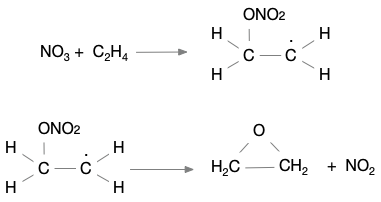
\includegraphics[width=0.75\textwidth]{NO3+C2H4.png}
\caption{Reacción del eteno con nitrato}
\label{no3c2h4}
\end{center}
\end{figure}
Así, los epóxidos (epoxietano en el caso de \ce{C2H4}) se forman a partir de los aductos de \ce{NO3}--alqueno. La vida del aducto es lo suficientemente larga como para permitir la rotación molecular alrededor del enlace C-C, y los epóxidos cis y trans se forman en la misma proporción independientemente de si se comienza con alquenos cis o trans asimétricos, como cis y trans-2-. buteno.

Mientras tanto, el aducto \ce{NO3}--alqueno reacciona con el \ce{O2} en la atmósfera para formar un radical peroxi, a partir del cual se forma el dinitrato (\textbf{Figura~\ref{aducto}}).
\begin{figure}[htbp]
\begin{center}
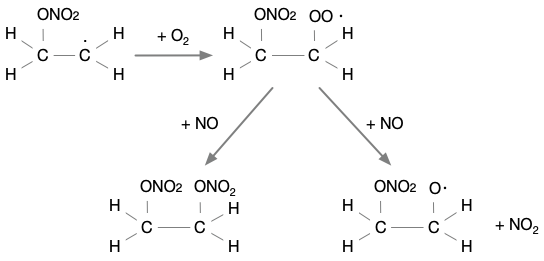
\includegraphics[width=0.75\textwidth]{AductoNO3.png}
\caption{Formación del dinitrato a partir de un aducto-NO$_3$}
\label{aducto}
\end{center}
\end{figure}

\item[\ce{NO3 + HCHO} ] 
\index{formadelhido@formaldehído}
El \ce{NO3} reacciona con aldehídos distintos de los alquenos entre los compuestos orgánicos. Dado que los radicales \ce{HO2} se forman a partir de radicales acilo (RCO) generados en la reacción, las reacciones de aldehídos \ce{NO3} son importantes como fuente de radicales HO y \ce{HO2} durante la noche. En este párrafo, se describen las reacciones del \ce{NO3} con HCHO y \ce{CH3CHO} como ejemplo representativo de aldehídos.

Las reacciones del \ce{NO3} y los aldehídos son la abstracción del átomo de H del grupo aldehído. En el caso de HCHO y \ce{CH3CHO}, las reacciones proceden como,
\reaction*{NO3 + HCHO -> HONO2 + HCO^.}
\reaction*{NO3 + CH3CHO -> HONO2 + HC3CO^.}
para producir radicales formilo\index{radical!formilo} y acetilo\index{radical!acetilo}, HCO y \ce{CH3CO}, respectivamente, a partir de los cuales se generan radicales peroxi, \ce{HO2} y \ce{CH3C(O)OO^.} al reaccionar  con el \ce{O2}.
\reaction*{HCO^. + O2 -> HO2  +  CO}
\reaction*{HC3CO^. + O2 ->[M]  CH3C(O)OO^.}
\end{description}

\subsection{Reacciones del ozono}
\index{ozono!reacciones troposfericas}
Aunque el ozono (\ce{O3}) es una especie reactiva entre las moléculas estables de la atmósfera, las moléculas asociadas a una reacción homogénea en fase gaseosa no son tantas. Las reacciones atmosféricas importantes son reacciones con átomos de halógeno en la estratosfera, NO, \ce{NO2}, OH y \ce{HO2} tanto en la troposfera como en la estratosfera, y alquenos (olefinas), dienos (diolefinas), e hidrocarburos cíclicos biogénicos, etc. en la troposfera. Entre ellas, las reacciones con NO, \ce{NO2} y \ce{C2H4} como alqueno típico se describen en detalle.

\begin{description}
\item[ \ce{O3 + NO}]
La reacción del \ce{O3} y el NO en la troposfera disipa el \ce{O3} temporalmente y se conoce como``reacción de titulación'',\index{ozono!titulacion@titulación} que es importante en fuentes cercanas de \ce{NO_$x$} y en el aire urbano. En la estratosfera, es importante como reacción que constituye  el ciclo de \ce{NO_$x$} para provocar la destrucción neta de \ce{O3}.

La reacción del \ce{O3} y el NO se puede escribir como,
\reaction*{O3 + NO -> NO2 + O2}
\item[ \ce{O3 + NO2}]
La reacción de \ce{O3} y \ce{NO2} es importante como reacción de formación de radicales \ce{NO3} en la química troposférica. Las reacciones del \ce{NO3} con otras especies atmosféricas se describe en otra sección.
\reaction*{O3 + NO2 -> NO3 + O2}

\item[ \ce{O3 + C2H4}]
Las reacciones importantes del  \ce{O3} en la atmósfera contaminada son aquellas con compuestos orgánicos con dobles enlaces como alquenos, dienos, terpenos, etc. Aquí se describen las reacciones elementales más fundamentales con el etileno (\ce{C2H4}).
\reaction*{O3 + C2H4 -> productos}
La energía de activación del \ce{O3} y la reacción del alqueno disminuye con el aumento del número de átomos de carbono y las constantes de velocidad de reacción aumentan rápidamente. Por ejemplo, la energía de activación para la reacción con propileno (\ce{C3H6}) y $\alpha$-pineno (\ce{C10H16}) disminuye a $15.6$ y $4.8\kilo\joulepermolenp$, y las constantes de velocidad son $1.0\times10^{17}$ y $9.0\times10^{17}\centi\cubic\metre$ molécula$^{-1}$, respectivamente, que son de uno a dos órdenes de magnitud más grandes que los del etileno.

Se sabe que la reacción inicial del \ce{O3} y los alquenos es la formación de compuestos carbonílicos y óxido de carbonilo a través del ozonuro primario formado por la adición cíclica de \ce{O3} al doble enlace. En el caso del etileno, la fórmula de reacción se puede representar como se muestra en la \textbf{Figura~\ref{ozonido}}:
\begin{figure}[htbp]
\begin{center}
%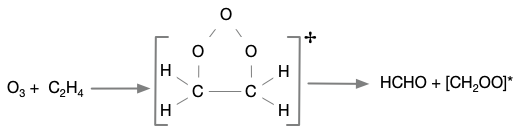
\includegraphics[width=0.75\textwidth]{ozonido.png}
\begin{picture}(100,24)
\put(1,8){\ce{O3 +C2H4 ->}}
% Hidrogenos izquierda
\put(26,3){H}
\put(26,15){H}
% lineas izquierda ozonido
\put(28,6){\line(5,3){4.4}}
\put(28,14){\line(5,-3){4.4}}
\put(34.2,11.7){\line(0,1){2}}
\put(34.2,17.5){\line(5,3){4}}
% Carbono izquierdo
\put(33,9){C}
\put(33,14){O}
% Oxigeno centro superior
\put(38.5,19){O}
% linea derecha del oxigeno central
\put(45.2,17.5){\line(-5,3){4}}
% Hidrogeno derecha
\put(46.2,11.7){\line(0,1){2}}
\put(52,3){H}
\put(52,15){H}
\put(45,14){O}
\put(45,9){C}
% enlace carbono carbono
\put(36,10){\line(1,0){8}}
% corchete izquierdo
\put(25,2){\line(0,1){20}}
\put(25,2){\line(1,0){2}}
\put(25,22){\line(1,0){2}}
% lineas derecha ozonido
\put(52,6){\line(-5,3){4.4}}
\put(52,14){\line(-5,-3){4.4}}
%corchete derecho
\put(56,2){\line(0,1){20}}
\put(54,2){\line(1,0){2}}
\put(54,22){\line(1,0){2}}
% parte 2 de la reacción
\put(55.5,8){\ce{-> HCHO + CH2OO^.}}
%
\put(56.3,20){$\dagger$}
%\put(0,0){\line(1,0){100}}
%\put(60,0){\line(0,1){24}}
\end{picture}
\caption{Reacción de ozono con etileno, con la formación de ozonido intermedio.}
\label{ozonido}
\end{center}
\end{figure}
La reacción conlleva a la formación de un ozónido ($\dagger$) en la fase gaseosa.

Las especies tipo RR'COO (\ce{CH2OO} en el caso de \ce{C2H4}) formadas por la descomposición del ozonuro\index{ozonuro} primario en la reacción de ozono-olefina se denominan en general óxido de carbonilo o intermedio de Criegee\index{criegge@\textbf{Crieege}}, por el nombre de Criegee, quien propuso por primera vez el mecanismo. En cuanto al intermedio Criegee, aunque la existencia de la especie ha sido bien reconocida, incluso en estudios teóricos, desde hace mucho tiempo no se realiza una medición directa en la fase gaseosa.
Se sabe que el \ce{CH2OO} producido en la reacción  está excitado por vibración, sufre parcialmente descomposición unimolecular y participa parcialmente en reacciones bimoleculares con otras moléculas en las condiciones atmosféricas como las presentadas en \textbf{Figura~\ref{ch2oo}}
\begin{figure}[htbp]
\begin{center}
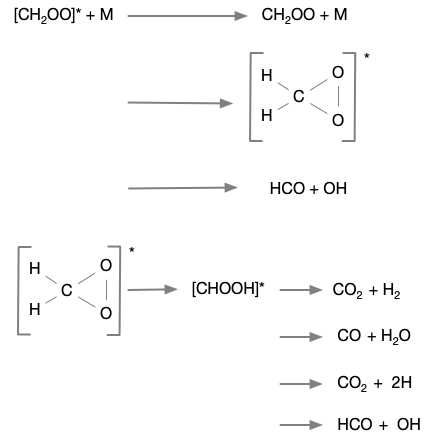
\includegraphics[width=0.65\textwidth]{ch2oo.png}
\caption{Reacciones del  \ce{CH2OO}.}
\label{ch2oo}
\end{center}
\end{figure}
\end{description}

\section{Oxidaci\'on de Compuestos Org\'anicos}
\index{COV!oxidacion@oxidación}
A medida que las actividades humanas continúan influyendo en la atmósfera, se observa un aumento en las concentraciones de sustancias de origen humano, como los óxidos de nitrógeno (\ce{NO_$x$} , que incluye NO y \ce{NO2} ) y los compuestos orgánicos volátiles (COV), superando ciertos umbrales críticos. Esta alteración conduce a una química troposférica que se encuentra más allá de los límites de la atmósfera natural. Se manifiestan reacciones químicas caracterizadas como ``reacciones del esmog''. En este contexto, se exploran los mecanismos de oxidación que involucran la interacción de \ce{NO_$x$}  y COV, directamente vinculados a la cadena de reacción del radical hidroxilo (OH).

\subsection{Reacciones en la troposfera}
Los procesos de reacción de oxidación de COV en presencia de \ce{NO_$x$}  son diferentes para alcanos (hidrocarburos saturados), alquenos (hidrocarburos insaturados con un doble enlace, también llamados olefinas), alquinos (hidrocarburos insaturados con un triple enlace) e hidrocarburos aromáticos (hidrocarburos insaturados). con un anillo de benceno). Sin embargo, todos los NMVOC reaccionan con OH y el ciclo de la cadena \ce{HO_$x$}  se puede expresar formalmente como,
\begin{eqnarray*}
\ce{OH + RH + O2& -> & RO2 + productos \\
RO2 + NO & -> & RO + NO2\\
RO + O2 & -> & R\textrm{'}CHO(R\textrm{'}COR\textrm{''}) + HO2 \\
HO2 + NO & -> & OH + NO2}
\end{eqnarray*}
tienen en común la mayoría de los NMVOC un mecanismo de forma similar al \ce{CH4}. En cuanto a los aldehídos, también se puede aplicar casi la misma forma del mecanismo de reacción en cadena. También son importantes las reacciones de oxidación con \ce{O3} y \ce{NO3} para los alquenos y la reacción con \ce{NO3}  para los aldehídos. En esta sección se resumen los mecanismos de reacción de oxidación de hidrocarburos y aldehídos con OH, \ce{O3} y \ce{NO3}.

\subsection{Mecanismo de oxidaci\'on de alcanos con OH}
\index{alcanos!oxidacion@oxidación con OH}

El proceso inicial de la reacción del alcano con OH es la extracción de hidrógeno, al igual que para el \ce{CH4}, y la extracción de hidrógeno del átomo de carbono primario, secundario y terciario es posible para un alcano con número de carbonos C3.

Como ejemplo de alcanos, el mecanismo de reacción de oxidación del n-butano (\ce{n-C4H10}) por OH en presencia de \ce{NO_$x$}  se muestra en la \textbf{Figura~\ref{butanOH}}

\begin{figure}[htbp]
\begin{center}
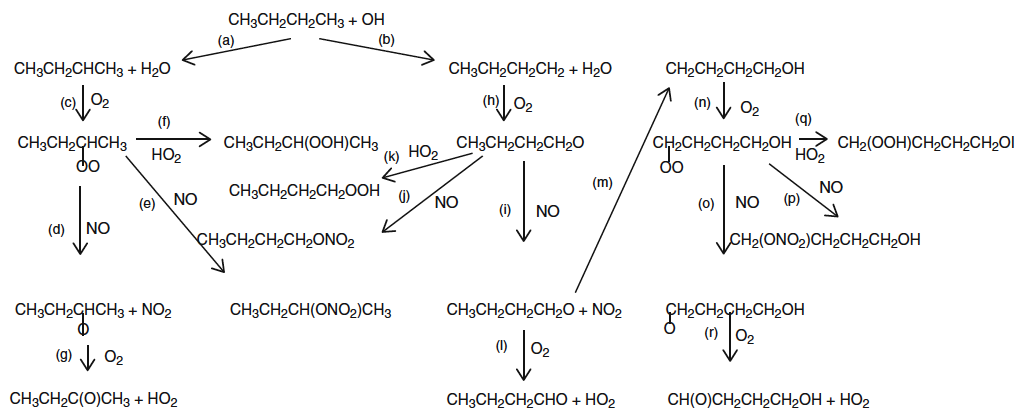
\includegraphics[width=0.97\textwidth]{butanoOH.png}
\caption{Reacciones del  butano con el OH.}
\label{butanOH}
\end{center}
\end{figure}

En el caso del n-butano, el radical 2-butilo y 1-butilo se forma mediante el proceso de abstracción (a) del carbono secundario y (b) del carbono primario, respectivamente. En general, la probabilidad de reacción aumenta para el carbono primario<secundario<terciario, lo que refleja la disminución de la energía del enlace. La relación del proceso (a) y (b) es ca. 85 y 15\% en el caso del n-butano a $298\kelvin$.

Los radicales alquilo formados por la reacción de abstracción reaccionan exclusivamente con \ce{O2} en la atmósfera para formar radicales alquilperoxi (vías (c) (h)), y la mayoría de ellos luego se transforman en radicales alcoxi oxidando NO a \ce{NO2} en presencia de \ce{NO$_x$} (vías (d) e (i)). Sin embargo, algunos radicales alquilperoxi reaccionan con NO mediante las reacciones de isomerización por recombinación (e) y (j), para formar nitrato de alquilo.

Aunque los rendimientos de nitrato de 2-butilo y 1-butilo no son grandes en el caso de los radicales 2-butilo y 1-butilo, los rendimientos de producción de nitratos de alquilo aumentan con el aumento del número de carbonos de los radicales alquilo. Dado que estas reacciones actúan como reacciones de terminación. ara la reacción en cadena del OH, son importantes como parámetros para determinar la eficiencia de la formación de ozono en los cálculos del modelo. 

Los radicales 2-butoxi y 1-butoxi formados en las reacciones de los radicales 2-butilo y 1-butilperoxi con NO (rutas (d) y (j)), reaccionan con \ce{O2}  para producir \ce{HO2}  junto con compuestos carbonílicos como el metilo. etilcetona y butanal (ruta (g) y (l)), y completar el ciclo \ce{HO$_x$}. Bajo las concentraciones típicas de \ce{NO$_x$} en la atmósfera contaminada, la velocidad de formación de nitratos de alquilo mediante reacciones de radicales alcoxi con \ce{NO2}  es insignificante; la reacción de isomerización por recombinación de los radicales alquilperoxi con NO es la vía principal como proceso de formación de nitrato de alquilo. Se sabe que para los radicales alcoxi de cadena lineal con un número de carbonos?4, como los radicales 1-butoxi, la isomerización forma radicales alcoxi en radicales alcohol, aunque pueden ocurrir anillos de seis miembros como se observa en la \textbf{Figura~\ref{butcic}}
\begin{figure}[htbp]
\begin{center}
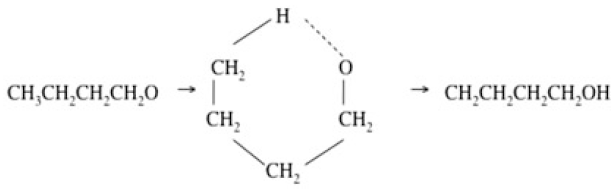
\includegraphics[width=0.97\textwidth]{butano-ciclico.png}
\caption{Isomerización del  1-butoxi}
\label{butcic}
\end{center}
\end{figure}

En la \textbf{Figura~\ref{butcic}}, la vía (m) corresponde a este proceso, y los radicales n-butanol formados producen hidroxibutanal y nitrato de 1-hidroxibutilo siguiendo un proceso similar al de los radicales butilo mencionados anteriormente (vías (r) y (p). respectivamente).

Además, en cuanto a los radicales alcoxi con un número de carbonos C4, se sabe que se produce el siguiente tipo de descomposición unimolecular para romper el enlace C-C entre el carbono unido al grupo carboxilo y el átomo de carbono adyacente.
\reaction*{RCH(O)R\textrm{'} -> RCHO + R\textrm{'} }

En condiciones relativamente bajas de NOx en la atmósfera, una parte de los radicales alquil peroxi y los radicales hidroxialquil peroxi reaccionan con HO2 para dar hidroperoxibutano (vías (f), (k)) e hidroxihidroperoxibutano (vía (q)). Así, en las reacciones de oxidación de alcanos en la atmósfera, además de los aldehídos, cetonas y nitratos de alquilo normales, también podrían producirse hidroperóxidos, hidroxihidroperóxidos y nitrato de hidroxialquilo.

\subsection{Mecanismo de oxidaci\'on de alquenos con OH}
\index{alquenos!oxidacion@oxidación con OH}

Las reacciones iniciales de alquenos y OH son la adición, y en su mayoría se encuentran en el límite de alta presión en condiciones atmosféricas, incluido el etileno, como se vió anteriormente. La reacción de adición forma radicales $\beta$-hidroxialquilo que tienen un grupo OH en el carbono adyacente al átomo de carbono con un electrón desapareado.
\reaction*{OH + RCH\bond{=}CH2 -> RCH-CH2OH o RCH(OH)-CH2 }
Para alquenos asimétricos con número de carbonos C3, existe la posibilidad de que el OH se agregue a cualquiera de los extremos del doble enlace como se muestra arriba.

\begin{figure}[htbp]
\begin{center}
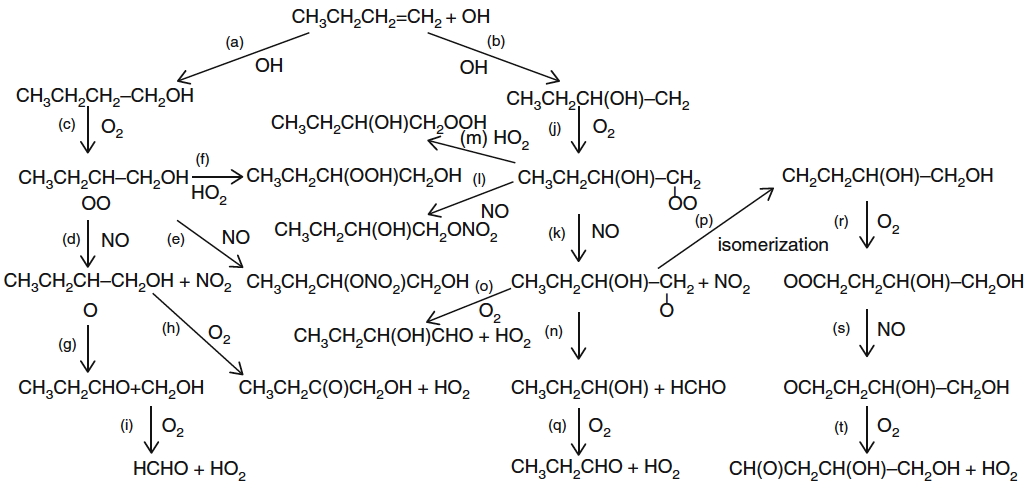
\includegraphics[width=0.97\textwidth]{buteno-OH.png}
\caption{Secuencia de reacciones del 1-buteno con OH}
\label{butenOH}
\end{center}
\end{figure}

La \textbf{Figura~\ref{butenOH}} resume el mecanismo de reacción del 1-buteno (1-\ce{C4H8}) como ejemplo de alquenos. Los radicales hidroxialquilo formados por las rutas (a) y (b) son un tipo de radicales alquilo mencionados en la sección anterior y forma exclusivamente radicales hidroxiperoxi por reacción con el \ce{O2} de la atmósfera.

De los radicales hidroxiperoxi, los radicales oxi (radicales hidroxibutoxi) y \ce{NO2} (vías (d), (k)), y parcialmente nitrato de hidroxibutilo (vías (e), (l)) se producen por reacción con NO como en el caso de los radicales alquilperoxi descritos en el párrafo anterior. Los rendimientos de nitratos de hidroxialquilo son del 2 al 6\% para los alquenos C4-C6 (O’Brien et al. 1998), que es aproximadamente la mitad de los de los nitratos de alquilo de los radicales alcoxi. Se sabe que los radicales hidroxialcoxi formados en las vías (d) y (k) siguen las tres vías de reacción: descomposición unimolecular ((g), (n)), abstracción de átomos de H por \ce{O2} ((h), (o)), y formación de radicales dihidroxilo por isomerización (p).

En el caso de los oxirradicales, respectivamente. En la vía de descomposición unimolecular se forman compuestos carbonílicos (\ce{CH3CH2CHO}, \ce{HCHO}) con menos átomos de carbono que un reactivo y radicales hidroxialquilo (\ce{CH2OH}, \ce{CH3CHOH}). A partir de los radicales hidroxialquilo se produce \ce{HO2} mediante la reacción del \ce{O2}. A partir de la reacción de abstracción del átomo de H por el \ce{O2}, se forman radicales hidroxicetona, hidroxialdehído y \ce{HO2}. A partir de los radicales \ce{HO2}, el OH se reproduce mediante la reacción de \ce{HO2} y NO de modo que se completa el ciclo \ce{HO_$x$}.

Los radicales hidroxialcoxi formados en la vía (k) pueden tener lugar por isomerización mediante desplazamiento intramolecular del átomo de H a través de un anillo de seis miembros como en el caso del radical alcoxi del párrafo anterior. Luego, el dihidroxialdehído se forma en las vías (q), (r), (s) a través de radicales dihidroxilo que tienen dos grupos OH en una molécula. La formación de dihidroxil aldehído se ha confirmado en experimentos de laboratorio, y el rendimiento de dihidroxil aldehído (3,4-dihidroxil butanal) es de 0.04 para 1-buteno, pero llega hasta 0.6 para 1-octeno. En bajas concentraciones de \ce{NO_$x$}, una parte de los radicales hidroxiperoxi reacciona con \ce{HO2} y se sabe que produce hidroxihidroperoxibutano (vías (f), (m)).

Por lo tanto, se cree que las reacciones de oxidación de alquenos con OH en la atmósfera contaminada dan como resultado varios nitratos e hidroperóxidos orgánicos, como hidroxinitrato, nitrato de dihidroxilo, hidroxihidroperóxido e hidroperóxido de dihidroxilo.

Esto sugiere que hay muchos peróxidos orgánicos y nitratos orgánicos no detectados y no identificados en la atmósfera contaminada junto con los productos de oxidación OH de los alcanos discutidos en el párrafo anterior.

\subsection{Mecanismo de oxidaci\'on de alquenos con NO$_3$}
\index{alquenos!oxidacion@oxidación con NO$_3$}
Las reacciones iniciales del \ce{NO3} y los alquenos son la adición de dobles enlaces como se vió en el capitulo anterior. Las constantes de velocidad de reacción aumentan con el número de carbonos, pero para la misma especie con número de carbonos las de los alquenos internos son mucho mayores. Los mecanismos de reacción de las reacciones de \ce{NO3}-alqueno son similares a aquellas con OH y alquenos y a continuación se puede ilustrar un ejemplo para cis-2-buteno.
\begin{figure}[htbp]
\begin{center}
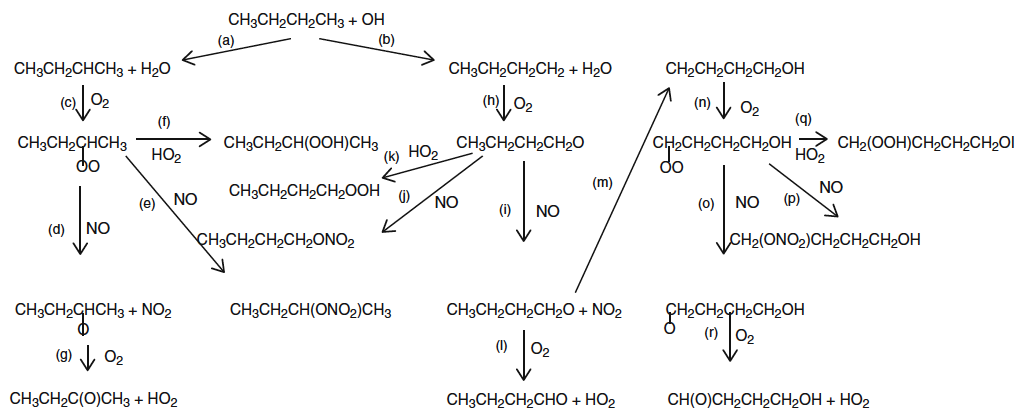
\includegraphics[width=0.97\textwidth]{butanoOH.png}
\caption{Oxidación del cis-2-buteno con NO$_3$.}
\label{buteNO3}
\end{center}
\end{figure}

\subsection{Mecanismo de oxidaci\'on del isopreno}
El isopreno (\ce{CH2=C(CH3)-CH=CH2}) es llamado 2-metil-1,3-butadieno por la nomenclatura de la IUPAC, un compuesto con dos dobles enlaces en una molécula, y es el hidrocarburo biogénico más importante, que representa representan el 50\% de las emisiones globales (Guenther et al. 2006). Las constantes de velocidad del isopreno son grandes, $1.0\times10^{-11}, 1.3\times10^{-17} $ y $6.8\times10^{-13} \centi\cubic\metre$  molécula$^{-1}$ s$^{-1}$ a $298\kelvin$ para OH, \ce{O3} y \ce{NO3}, respectivamente. Las reacciones de cualquiera de estas especies son importantes en la atmósfera, particularmente aquellas con OH y \ce{O3} durante el día y con \ce{NO3} durante la noche.

Los mecanismos de oxidación del isopreno con OH, \ce{O3} y \ce{NO3} son reacciones de adición similares a los alquenos y pueden considerarse como una aplicación de las reacciones descritas en la sección anterior. Sin embargo, dado que el isopreno tiene dos dobles enlaces asimétricos, se deben considerar cuatro vías de reacción dependiendo de la adición de especies activas a cualquiera de los dobles enlaces y a cada lado de los carbonos. Se han realizado muchos estudios experimentales y teóricos sobre el mecanismo de oxidación del isopreno (Finlayson-Pitts y Pitts 2000; Seinfeld y Pandis 2006), y Fan y Zhang (2004) presentaron el esquema de reacción para cada uno de OH, \ce{O3} y \ce{NO3} resumiendo esos estudios. Los esquemas de reacción siguientes  ilustran el mecanismo de reacción de oxidación del isopreno iniciado por OH, \ce{O3} y \ce{NO3}, respectivamente, adaptados de Fan y Zhang (2004).

\begin{figure}[htbp]
\begin{center}
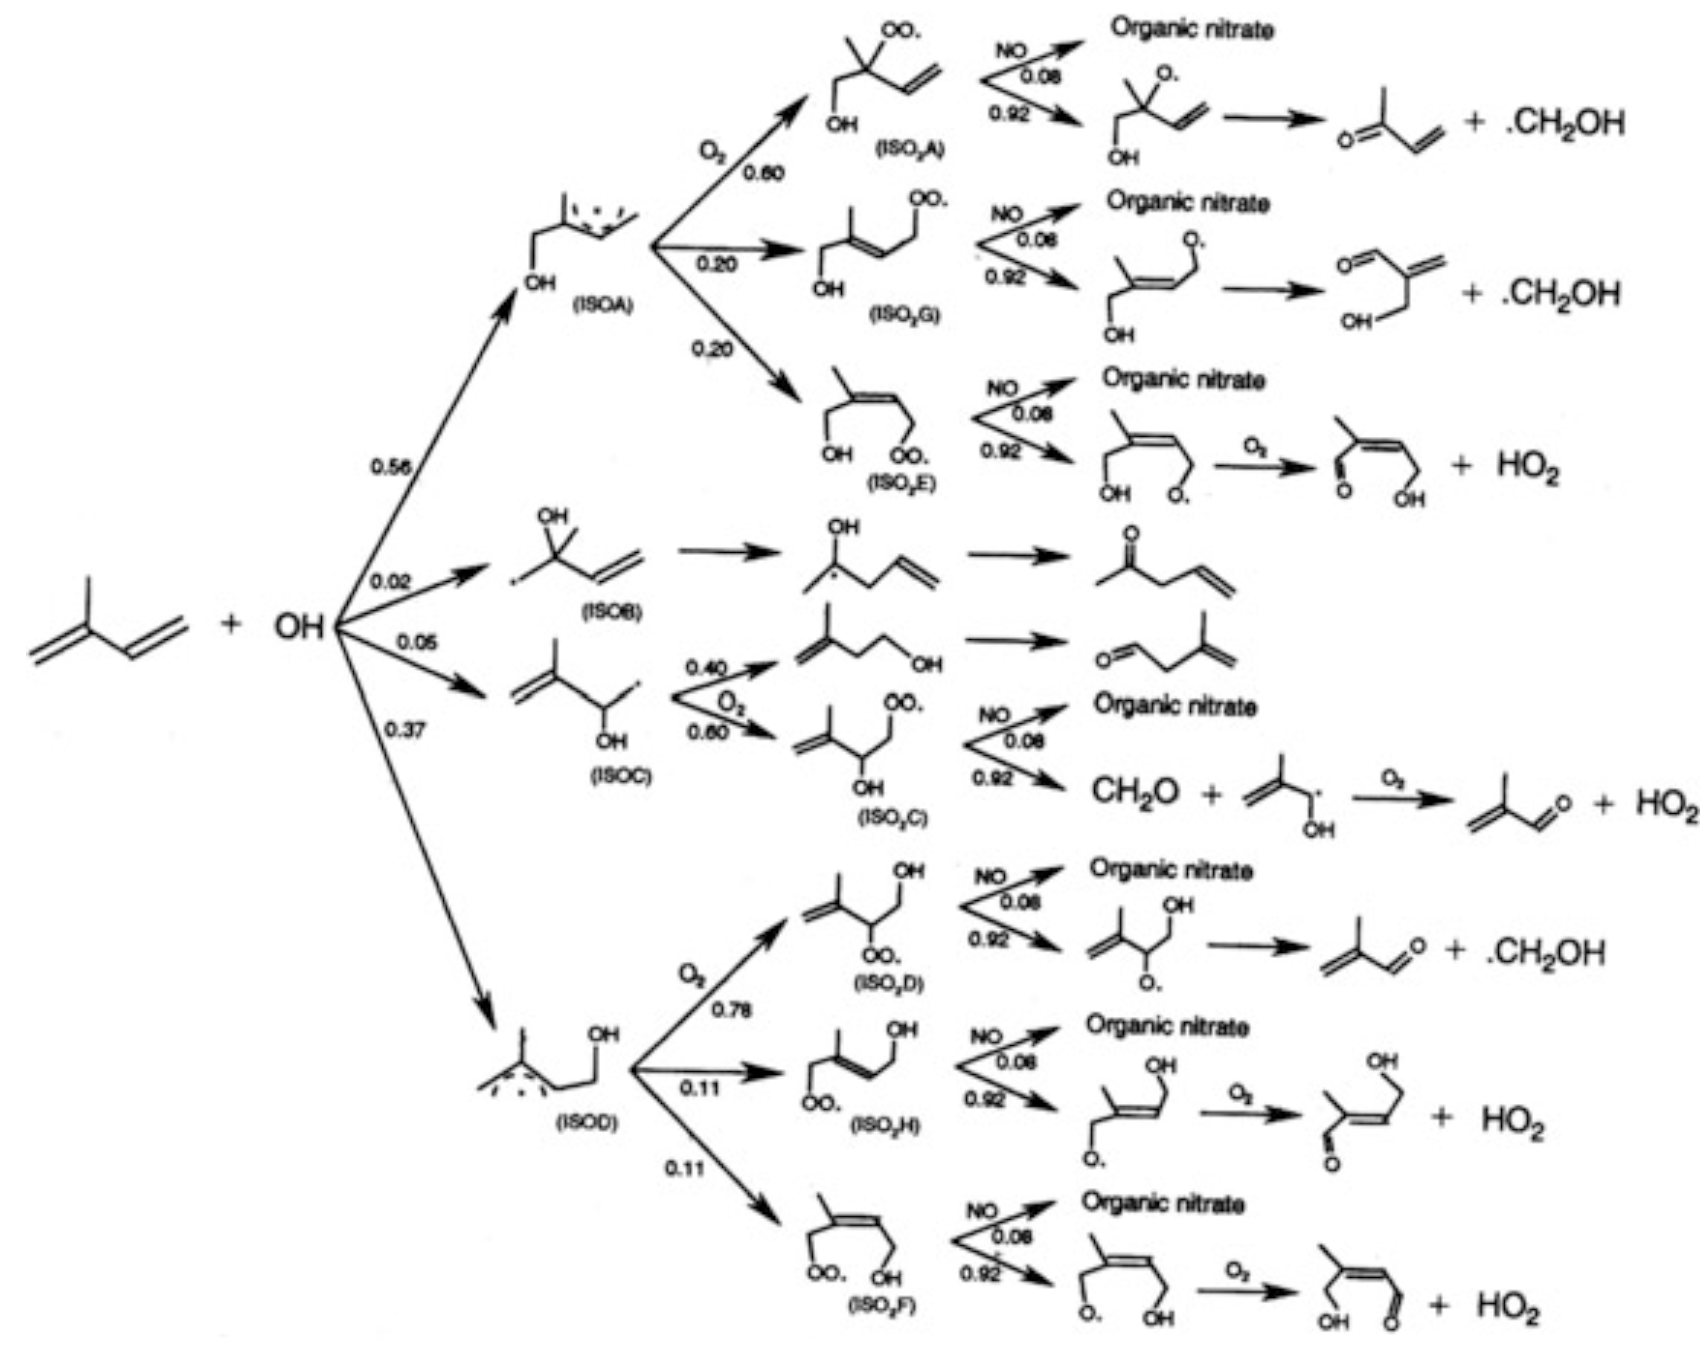
\includegraphics[width=0.97\textwidth]{isopreno-OH.png}
\caption{Oxidación del isopreno con OH.}
\label{isopOH}
\end{center}
\end{figure}

\begin{figure}[htbp]
\begin{center}
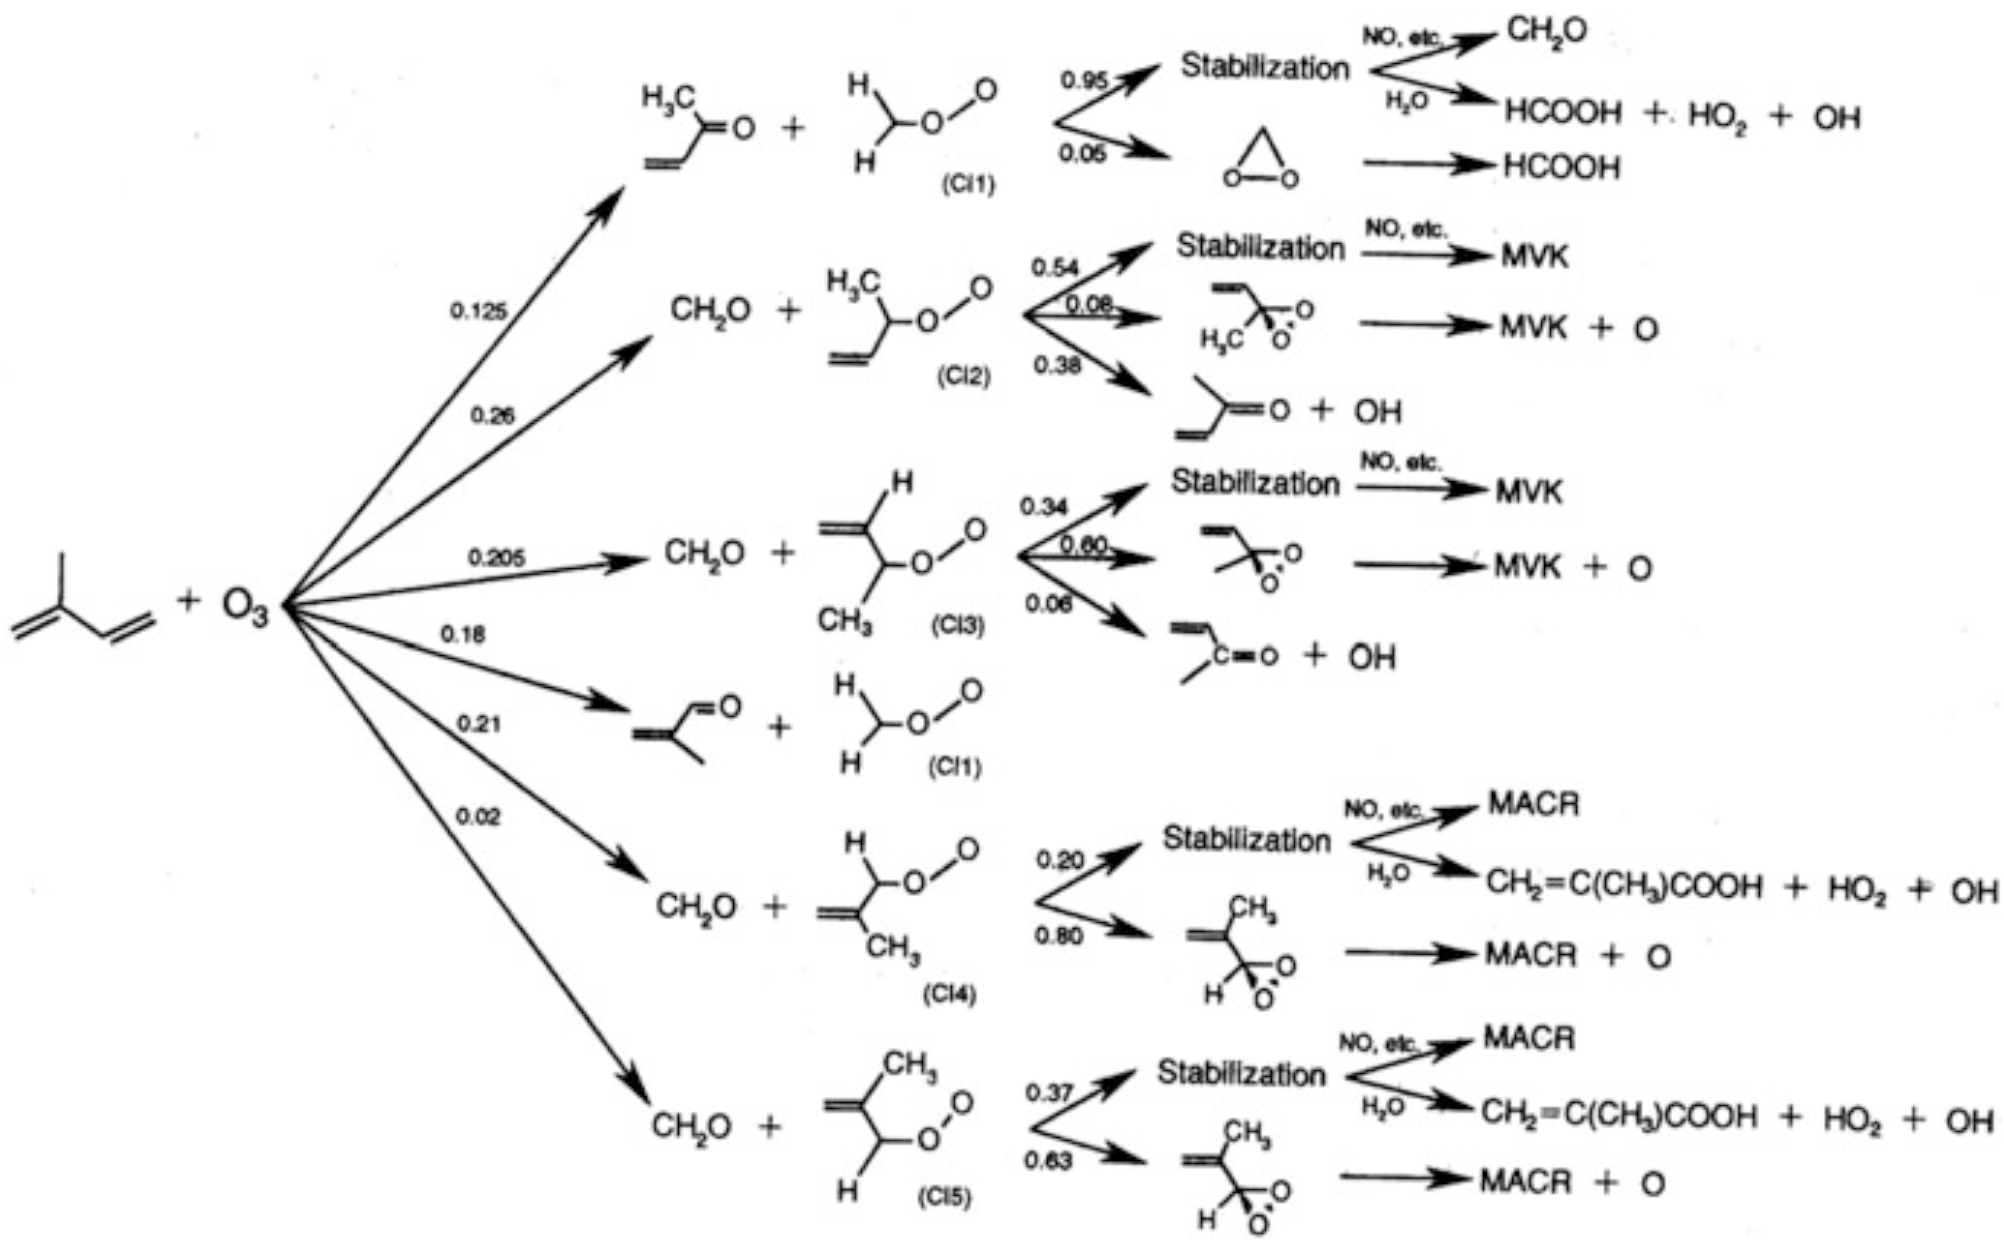
\includegraphics[width=0.97\textwidth]{Isopreno-Ozono.png}
\caption{Oxidación del isopreno con O$_3$ en presencia de NO$_x$.}
\label{isopO3}
\end{center}
\end{figure}
 
 \begin{figure}[htbp]
\begin{center}
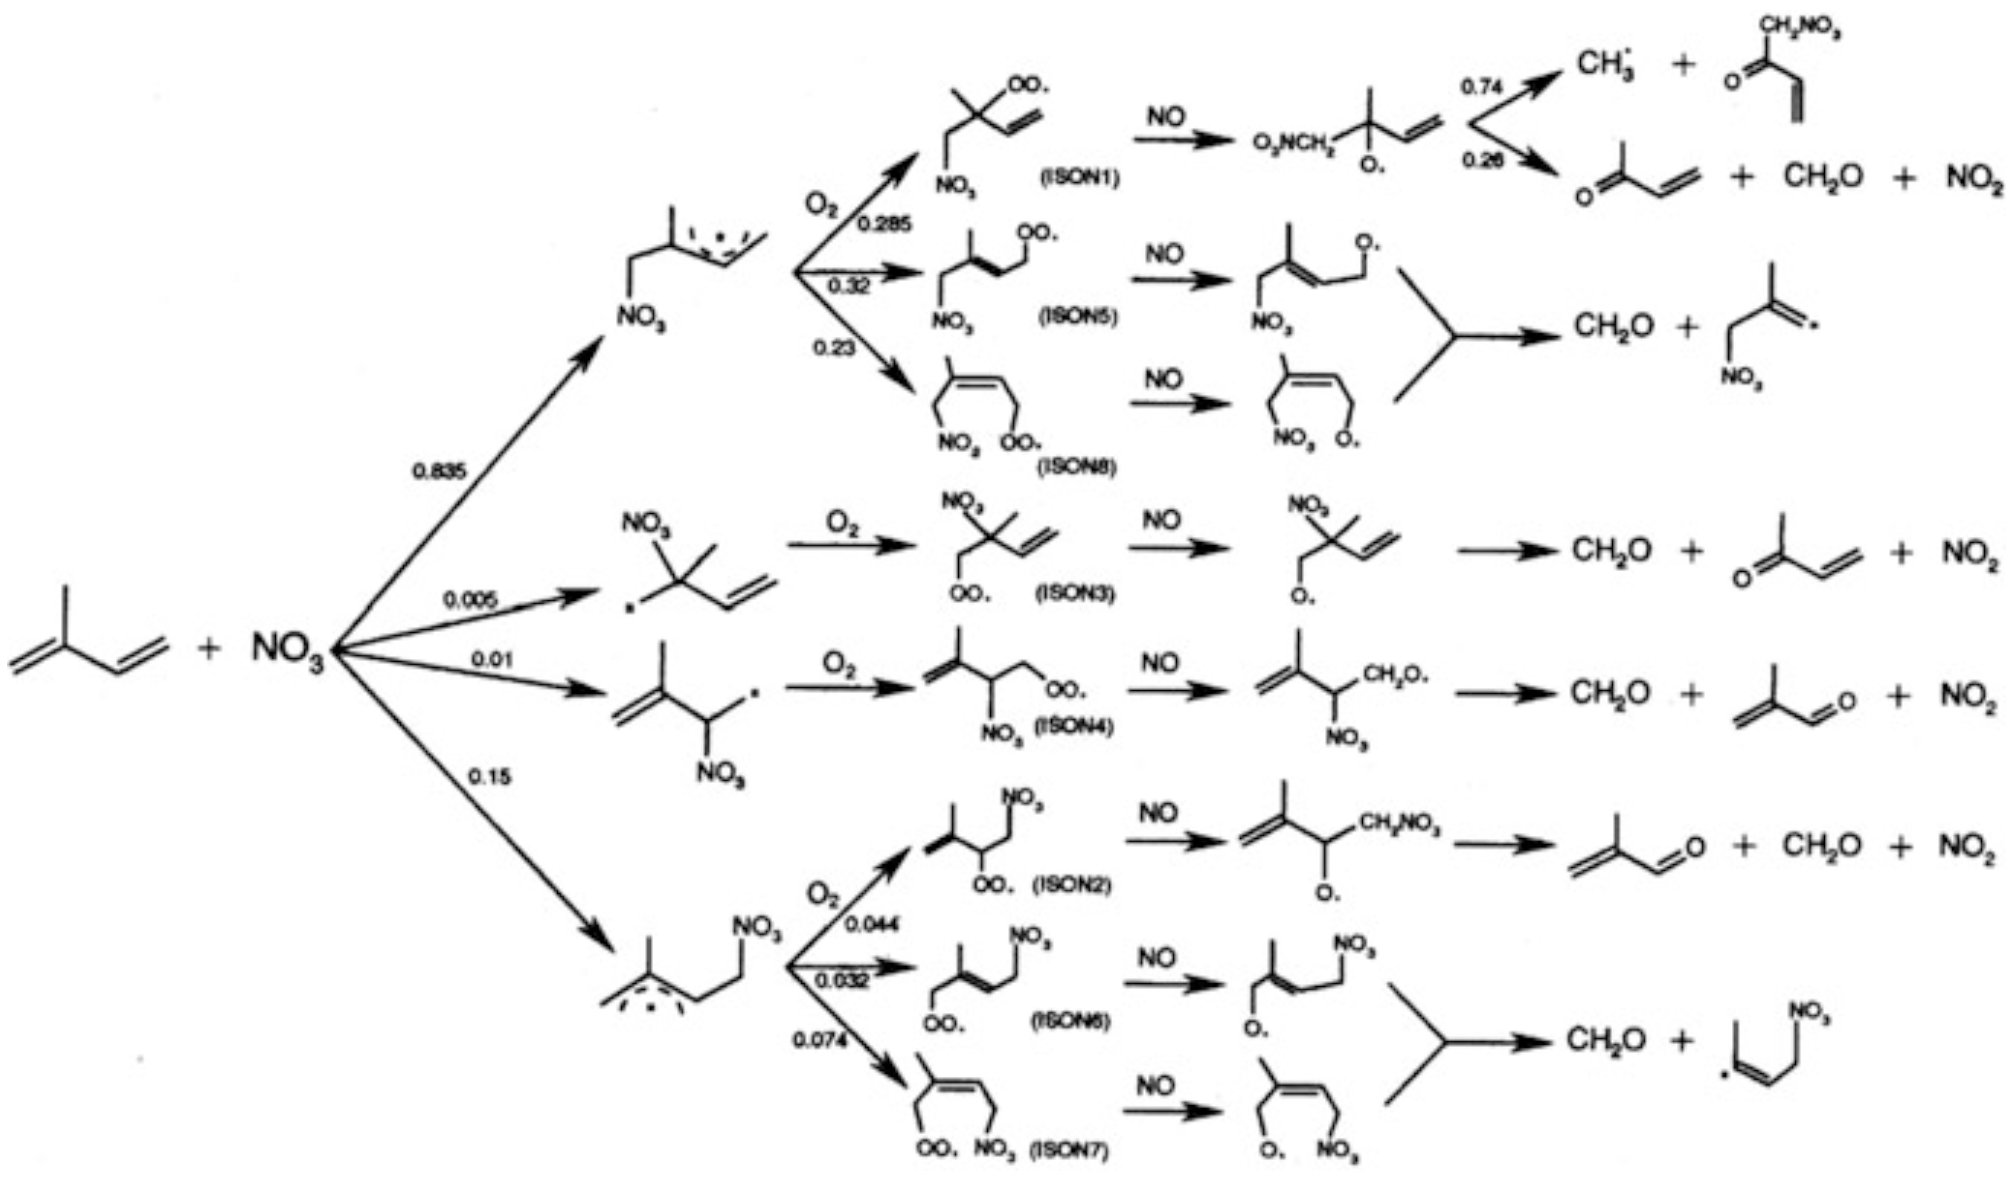
\includegraphics[width=0.97\textwidth]{Isopreno-NO3.png }
\caption{Oxidación del isopreno con NO$_3$.}
\label{isopNO3}
\end{center}
\end{figure}

Como se puede observar en el Esquema de Reacción con OH (\textbf{Figura~\ref{isopOH}}), los principales productos de la reacción de oxidación del isopreno por OH son la metacroleína (\ce{CH2\bond{=}CH(CH3)CHO}, MACR)\index{metacroleina}\index{MACR} y la metil vinil cetona (\ce{CH3C(O)CH\bond{=}CH2}, MVK)\index{MVK} (Karl et al. 2006). Además de ellos, como productos característicos se forman compuestos de hidroxicarbonilo insaturados y nitrato de hidroxi.

En la reacción de isopreno y \ce{O3} (\textbf{Figura~\ref{isopO3}} ), a través de cinco tipos de óxidos de carbonilo (intermedios de Criegee), se forman MACR y MVK como productos principales, como en el caso de la reacción de oxidación por OH, así como HCHO, HCOOH y ácidos carboxílicos insaturados. En esta reacción, similar a la reacción del alqueno y \ce{O3}, se forman radicales OH, lo cual es importante como fuente nocturna de OH.

En la reacción de isopreno con \ce{NO3} (\textbf{Figura~\ref{isopNO3}}), las reacciones transcurren a través de ocho tipos de radicales nitrooxialquilperoxi (ISON1-ISON8) y ocho tipos de radicales nitrooxialcoxi (ISN1-ISN8) formados a partir de los primeros por la reacción con NO. Los principales productos finales son formaldehído, aldehídos insaturados, cetonas y nitratos orgánicos, y los rendimientos de MACR, MVK son pequeños y diferentes de las reacciones con OH y \ce{O3}.

\subsection{Mecanismo de oxidaci\'on de alquinos con OH}
\index{alquinos!oxidacion@oxidación con OH}
En cuanto a la disipación atmosférica de los alquinos, el único proceso es la reacción con OH. Además, la reacción inicial de OH con alquinos es similar a la de los alquenos, y la reacción tiene lugar en el límite de alta presión de 1 atm para los alquinos con un número de carbonos superior a 3, aunque se necesitan varias atmósferas para alcanzar el límite de alta presión para acetileno (\ce{HC\bond{3}CH}). El principal alquino en la atmósfera contaminada es el \ce{C2H2} y su mecanismo de oxidación por OH se muestra en el esquema de reacción de la  \textbf{Figura~\ref{acetOH}}.

Como se ve en el esquema de reacción  el glioxal\index{glioxal} (CHO-CHO) es el producto principal del radical OH añadido en la reacción de OH y \ce{C2H2} a través de radicales peroxi y oxi. La vía de reacción principal produce \ce{HO2} en el último paso (e) y forma el ciclo de la cadena \ce{HO_$x$}. De manera similar, el metilglioxal (\ce{CH3COCHO}) y el biacetilo\index{biacetilo} (\ce{CH3COCH3CO}) se forman como productos principales a partir del propino (\ce{C3H4}) y 2-butino (\ce{2-C4H6}), respectivamente.
\begin{figure}[htbp]
\begin{center}
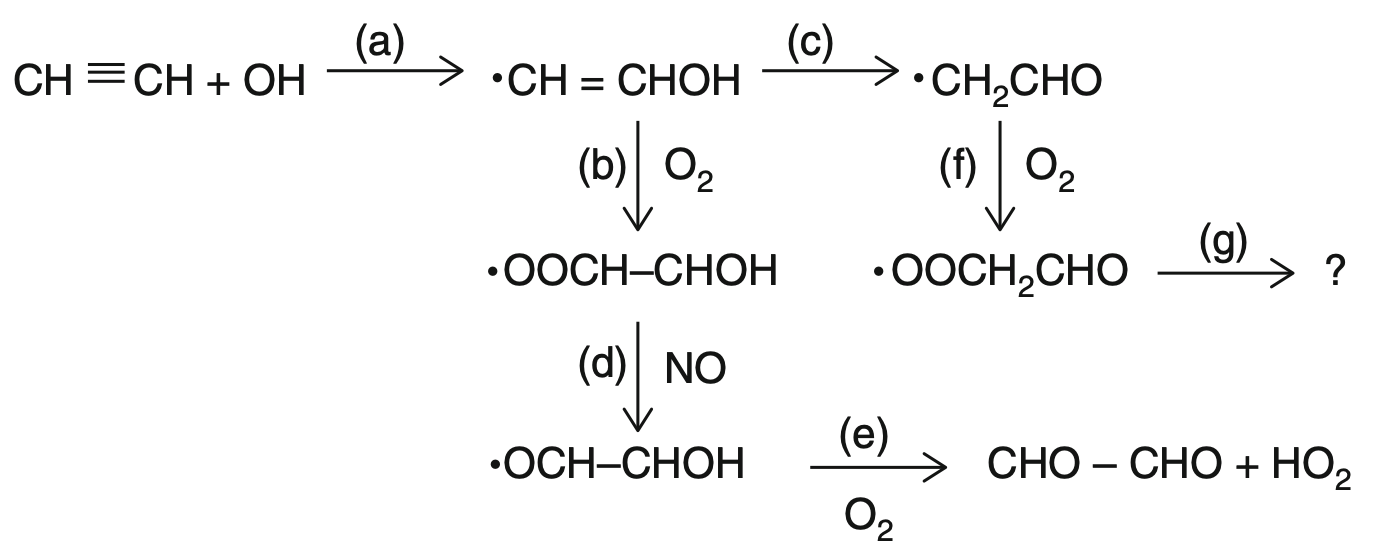
\includegraphics[width=0.97\textwidth]{Acetileno-OH.png }
\caption{Oxidación del acetileno con OH.}
\label{acetOH}
\end{center}
\end{figure}

Una parte del radical OH añadido se isomeriza como en la vía (c) y forma el radical vinoxi (\ce{CH2CHO}) (Schmidt et al., 1985), pero sus reacciones posteriores aún no se conocen bien.

\subsection{Mecanismo de oxidaci\'on de arom\'aticos con OH}
\index{aromaticos@aromáticos!oxidacion@oxidación con OH}

Las reacciones de OH e hidrocarburos aromáticos en condiciones atmosféricas constan de dos procesos, la adición al anillo de benceno y la abstracción del átomo de H del grupo alquilo. Aquí, tomando como ejemplo representativo el tolueno (\ce{CH3-C6H5}), cuya concentración es la más alta en general entre los hidrocarburos aromáticos en la atmósfera contaminada, la abstracción del átomo de H del grupo metilo de la cadena lateral da el radical bencilo de la siguiente manera 
\begin{figure}[htbp]
\begin{center}
\begin{picture}(50,20)
\put( 0  ,7  ){\ce{OH +}}
\put( 9  ,10  ){\line( 2, 1){4}}      % Enlace C-C sup izq(s)
\put( 9  , 5.5  ){\line( 0, 1){4.5}}  % Enlace C-C centro izq
\put( 9 , 5.5){\line( 2,-1){4}}       % Enlace C-C izq inf(i)
\put(17  ,10 ){\line(-2, 1){4}}       % Enlace C-C der sup
\put( 13.1, 12){\line( 0, 1){2}}       % Enlace del Metilo
\put(17  , 5.5){\line( 0, 1){4.5}}    % Enlace C-C centroder(d)
\put(17  , 5.5){\line(-2,-1){4}}      % Enlace C-C inf der
\put( 13.1, 7.8){\circle{6.3}}
\put(12, 15){{\footnotesize CH$_3$}}
\put(8,0){{\footnotesize Tolueno}}
\put(19 ,7.8){\vector( 1,0){9.5}}
\put( 30 ,10  ){\line( 2, 1){4}}      % Enlace C-C sup izq(s)
\put( 30, 5.5  ){\line( 0, 1){4.5}}  % Enlace C-C centro izq
\put( 30, 5.5){\line( 2,-1){4}}       % Enlace C-C izq inf(i)
\put(38 ,10 ){\line(-2, 1){4}}       % Enlace C-C der sup
\put(34.1, 12){\line( 0, 1){2}}       % Enlace del Metilo
\put(38  , 5.5){\line( 0, 1){4.5}}    % Enlace C-C centroder(d)
\put(38  , 5.5){\line(-2,-1){4}}      % Enlace C-C inf der
\put( 34.1, 7.8){\circle{6.3}}
\put(33, 15){{\footnotesize CH$_2\cdot$}}
\put( 39  ,7  ){\ce{+ H2O }}
\end{picture}
\caption{Oxidación del tolueno con OH.}
\label{TolOH}
\end{center}
\end{figure}

Se sabe que los principales productos del radical bencilo en presencia de \ce{NO_$x$} son el benzaldehído y el nitrato de bencilo (Akimoto et al. 1978; Klotz et al. 1998; Calvert et al. 2002; Atkinson y Arey 2003).
\begin{figure}[htbp]
\begin{center}
%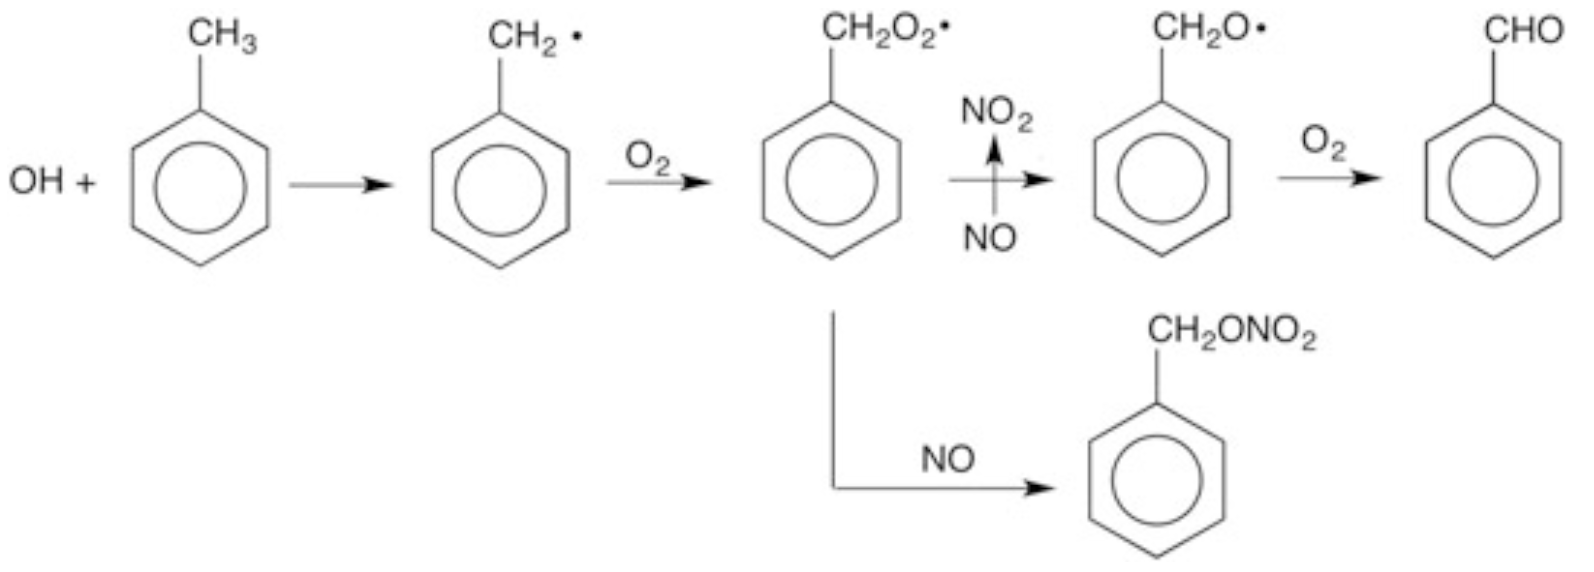
\includegraphics[width=0.97\textwidth]{Tolueno+OH+NOx.png }
\begin{picture}(100,40)
\put( 0  ,27  ){\ce{OH +}}
\put( 9  ,30  ){\line( 2, 1){4}}      % Enlace C-C sup izq(s)
\put( 9  ,25.5  ){\line( 0, 1){4.5}}  % Enlace C-C centro izq
\put( 9 , 25.5){\line( 2,-1){4}}       % Enlace C-C izq inf(i)
\put(17  ,30 ){\line(-2, 1){4}}       % Enlace C-C der sup
\put( 13.1, 32){\line( 0, 1){2}}       % Enlace del Metilo
\put(17  , 25.5){\line( 0, 1){4.5}}    % Enlace C-C centroder(d)
\put(17  , 25.5){\line(-2,-1){4}}      % Enlace C-C inf der
\put( 13.1, 27.8){\circle{6.3}}
\put(12, 35){{\footnotesize CH$_3$}}
%\put(8,0){{\footnotesize Tolueno}}
\put(19 ,27.8){\vector( 1,0){8.5}}
\put( 30 ,30  ){\line( 2, 1){4}}      % Enlace C-C sup izq(s)
\put( 30, 25.5  ){\line( 0, 1){4.5}}  % Enlace C-C centro izq
\put( 30, 25.5){\line( 2,-1){4}}       % Enlace C-C izq inf(i)
\put(38 ,30 ){\line(-2, 1){4}}       % Enlace C-C der sup
\put(34.1, 32){\line( 0, 1){2}}       % Enlace del Metilo
\put(38  , 25.5){\line( 0, 1){4.5}}    % Enlace C-C centroder(d)
\put(38  , 25.5){\line(-2,-1){4}}      % Enlace C-C inf der
\put( 34.1,27.8){\circle{6.3}}
\put(33, 35){{\footnotesize CH$_2\cdot$}}
\put( 39  ,27.8  ){\vector( 1,0){9.5}}
\put( 42 ,29  ){{\footnotesize  O$_2$}}
% despues de reaccionar con oxigeno
\put( 50 ,30  ){\line( 2, 1){4}}      % Enlace C-C sup izq(s)
\put( 50, 25.5  ){\line( 0, 1){4.5}}  % Enlace C-C centro izq
\put( 50, 25.5){\line( 2,-1){4}}       % Enlace C-C izq inf(i)
\put(58 ,30 ){\line(-2, 1){4}}       % Enlace C-C der sup
\put(54.1, 32){\line( 0, 1){2}}       % Enlace del Metilo
\put(58  , 25.5){\line( 0, 1){4.5}}    % Enlace C-C centroder(d)
\put(58  , 25.5){\line(-2,-1){4}}      % Enlace C-C inf der
\put(54.1,27.8){\circle{6.3}}
\put(53, 35){{\footnotesize CH$_2$O$_2\cdot$}}
\put(59  ,27.8  ){\vector( 1,0){9.5}}
\put(62  ,25.5 ){\vector( 0,1){6}}
\put(62.6 ,25 ){{\footnotesize NO}}
\put(62.6 ,30 ){{\footnotesize NO$_2$}}
% flecha hacia abajo
\put(54.1, 7.8){\line( 0, 1){14}}       %  Flecha hacia abajo
\put(54.1, 7.8){\vector( 1,0){14}}
\put( 59.5 ,8.5 ){{\footnotesize NO}}

\put( 70 ,10  ){\line( 2, 1){4}}      % Enlace C-C sup izq(s)
\put( 70, 5.5  ){\line( 0, 1){4.5}}  % Enlace C-C centro izq
\put( 70, 5.5){\line( 2,-1){4}}       % Enlace C-C izq inf(i)
\put(78 ,10 ){\line(-2, 1){4}}       % Enlace C-C der sup
\put(74.1, 12){\line( 0, 1){2}}       % Enlace del Metilo
\put(78  , 5.5){\line( 0, 1){4.5}}    % Enlace C-C centroder(d)
\put(78  , 5.5){\line(-2,-1){4}}      % Enlace C-C inf der
\put( 74.1, 7.8){\circle{6.3}}
\put(73, 15){{\footnotesize CH$_2$ONO$_2$}}
% despues de reaccionar con NO-NO2
\put( 70 ,30  ){\line( 2, 1){4}}      % Enlace C-C sup izq(s)
\put( 70, 25.5  ){\line( 0, 1){4.5}}  % Enlace C-C centro izq
\put( 70, 25.5){\line( 2,-1){4}}       % Enlace C-C izq inf(i)
\put(78 ,30 ){\line(-2, 1){4}}       % Enlace C-C der sup
\put(74.1,32){\line( 0, 1){2}}       % Enlace del Metilo
\put(78  , 25.5){\line( 0, 1){4.5}}    % Enlace C-C centroder(d)
\put(78  , 25.5){\line(-2,-1){4}}      % Enlace C-C inf der
\put(74.1,27.8){\circle{6.3}}
\put(73, 35){{\footnotesize CH$_2$O$\cdot$}}
\put(79  ,27.8  ){\vector( 1,0){9.5}}
\put(82 ,29  ){{\footnotesize  O$_2$}}
% despues de reaccionar con O2 segunda vez
\put( 90 ,30  ){\line( 2, 1){4}}      % Enlace C-C sup izq(s)
\put( 90, 25.5  ){\line( 0, 1){4.5}}  % Enlace C-C centro izq
\put( 90, 25.5){\line( 2,-1){4}}       % Enlace C-C izq inf(i)
\put(98 ,30 ){\line(-2, 1){4}}       % Enlace C-C der sup
\put(94.1, 32){\line( 0, 1){2}}       % Enlace del Metilo
\put(98  , 25.5){\line( 0, 1){4.5}}    % Enlace C-C centroder(d)
\put(98  , 25.5){\line(-2,-1){4}}      % Enlace C-C inf der
\put(94.1,27.8){\circle{6.3}}
\put(93, 35){{\footnotesize CHO}}
\end{picture}
\caption{Oxidación del tolueno con OH en presencia de  NO$_x$}
\label{TolOH2}
\end{center}
\end{figure}
De acuerdo con el esquema de reacción presentado en la \textbf{Figura~\ref{TolOH2}}, los radicales \ce{HO2} se forman de manera similar a los procesos de abstracción de átomos de H que forman alcanos. Dado que los radicales OH se regeneran a partir de \ce{HO2}, el ciclo de reacción en cadena de \ce{HO_$x$} se completa y el NO se oxida a \ce{NO2} simultáneamente.

\subsection{Mecanismo de oxidaci\'on de aldehídos con OH y NO$_3$}
\index{aldehidos@aldehídos!oxidacion@oxidación con OH y NO$_3$}
Las reacciones de oxidación de aldehídos con OH en presencia de \ce{NO_$x$} son muy importantes desde el punto de formar compuestos peculiares con fuerte toxicidad biológica llamados peroxiacilnitratos (PANs, \ce{RC(O)OONO2}). La reacción inicial de OH y aldehídos es la abstracción del átomo de H que forma el grupo aldehído para formar radicales acilo.

\begin{eqnarray}
\ce{CH3CHO + OH       & -> & CH3CO^. + H2O \nonumber\\
 CH3CO^. + O2             & ->[M] & CH3C(O)OO^. \label{VOC41}\\
 CH3C(O)OO^. + NO     &  -> &  CH3C(O)O^.  + NO2 \nonumber\\
 CH3C(O)OO^.  + NO2   & ->[M] &  CH3C(O)OONO2  \nonumber\\
 CH3C(O)O^.                  & -> &  CH3^. + CO2  \nonumber\\
   CH3^. + O2                 & ->[M] & CH3O2   \nonumber\\
  CH3O2 + NO                & -> &  CH3^. + NO2  \nonumber\\
   CH3O + O2                 & -> & HCHO  \label{VOC42} }
\end{eqnarray}
Estas vías de reacción son paralelas a las de los alcanos mencionados anteriormente  y las reacciones (\textbf{Figura~\ref{butanOH}}) después de que se formen radicales \ce{CH3} en la reacción  son las mismas que en los procesos de oxidación del metano descritos previamente. La característica específica de las reacciones de oxidación de aldehídos es la formación de nitratos de peroxiacilo metaestables a partir de la reacción de radicales peroxiacilo con \ce{NO2} mediante reacción (\ref{VOC41}). En el caso del acetaldehído, se forma nitrato de peroxiacetilo, \ce{CH3C(O)OONO2}. Este compuesto se llama PAN (nitrato de peroxiacetilo)\index{PAN} y se sabe que tiene una toxicidad para las plantas mucho más fuerte que el ozono. Un grupo de nitratos de peroxiacilo se denominan colectivamente PANs.

La reacción del aldehído con \ce{NO3} es la abstracción del átomo de H (Mora-Diez y Boyd, 2002), al igual que con el OH, y por ejemplo, en el caso del \ce{CH3CHO}
\reaction*{CH3CHO + NO3 -> CH3CO + HONO2}

Por lo tanto, las reacciones siguientes son las mismas que la reacción y las siguientes descritas anteriormente, y se forma \ce{HO2} mediante la reacción (\ref{VOC42}). Por tanto, la reacción del aldehído y el \ce{NO3} es importante como fuente nocturna de radicales \ce{HO$_x$}.
